% % \documentclass{article}
% % \usepackage[nonatbib,preprint]{neurips_2020}

% % \usepackage[utf8]{inputenc} % allow utf-8 input
% % \usepackage[T1]{fontenc}    % use 8-bit T1 fonts
% % \usepackage{hyperref}       % hyperlinks
% % \usepackage{url}            % simple URL typesetting
% % \usepackage{booktabs}       % professional-quality tables
% % \usepackage{amsfonts}       % blackboard math symbols
% % \usepackage{nicefrac}       % compact symbols for 1/2, etc.
% % \usepackage{microtype}      % microtypography

% % \usepackage{todonotes}
% % \usepackage[ruled,vlined]{algorithm2e}
% % \usepackage{amsmath}
% % \usepackage{graphicx}
% % \usepackage{geometry}                		     
% % \usepackage{mathtools}
% % \usepackage{amssymb}
% % \usepackage{bm,amsbsy}
% % \usepackage[sort&compress,numbers]{natbib}
% % \usepackage[space]{grffile} % for spaces in figs

% % \usepackage{tikz}
% % \usetikzlibrary{fit,positioning}
% % \usetikzlibrary{arrows.meta,shapes,tikzmark,calc}

% % \tikzstyle{every picture}+=[remember picture]
% % \tikzstyle{na} = [baseline=-.5ex]

% %  \include{m.symbols}
% % \newcommand\scalemath[2]{\scalebox{#1}{\mbox{\ensuremath{\displaystyle #2}}}}

% % \allowdisplaybreaks

% \documentclass[12pt]{article}
% \usepackage[utf8]{inputenc}
% \usepackage{tikz}
% \usepackage[utf8]{inputenc}
% \usepackage[scaled]{helvet}
% \usepackage[T1]{fontenc}
% \renewcommand\familydefault{\sfdefault}

% \tikzset{
%     box/.style={
%         anchor=north west,
%         minimum width=70mm, 
%         minimum height=36mm, 
%         text width=65mm, 
%         draw=black
%     }
% }

% \begin{document}%
% \centering

% \foreach \x in {3,...,4}
%     %%%%%%%%%% FIGURE: TASK SCHEMATIC smaller version %%%%%%%%%%%%%%%
%     \begin{tikzpicture}
%     \centering
%     \hspace{-0.5cm}
%     \begin{minipage}{\linewidth}
%     \vspace{-0.25cm}
%     \tikzset{every node}=[font=\sffamily]
% 	% INPUTS
%     \node[anchor=west] (fix) at (-10,3) {\includegraphics[trim=0mm 0mm 0mm 0mm, clip, width=0.3\linewidth]{figs/lesion 3/perf_change_delayanti.pdf}};
%     % \node[anchor=north] (h_diff) at ([shift={(2.5,1.2)}]fix.east) {\includegraphics[trim=0mm 0mm 0mm 0mm, clip,width=0.5\linewidth]{figs/lesion \x/h_diff_dmcnogo.pdf}};
%     % \node[anchor=north] (single) at ([shift={(0,0)}]h_diff.south) {\includegraphics[trim=0mm 0mm 0mm 0mm, clip, width=0.4\linewidth]{figs/lesion \x/single_unit_activations_delayanti.pdf}};
%     % \node[anchor=north] (pc_contribution) at ([shift={(0,0)}]single.south) {\includegraphics[trim=0mm 0mm 0mm 0mm, clip,width=0.5\linewidth]{figs/lesion \x/pc_contribution_delayanti.pdf}};
%     % \node[font=\bfseries] at ([shift={(0,1.3)}]fix.west) {A};
%     % \end{minipage}\hspace{-4.cm}
%     % \begin{minipage}{0.26\linewidth}
%     % \vspace{-0.6cm}
%     % \end{minipage}
%     % \vspace{-0.5cm}
%     \end{tikzpicture}
% %%%%%%%%%%%%%%%%%%%%%%%%%%%%%%%%%%%%%%%%%%%%%%%%%%%%%%%%%%%%%%%%%%%%%%%%%%%%%%%%%%%%%%%%%

% \end{document}


\documentclass[12pt]{article}
\usepackage[utf8]{inputenc}




\usepackage{tikz}

\usepackage[utf8]{inputenc}

\usepackage[scaled]{helvet}
\usepackage[T1]{fontenc}
\renewcommand\familydefault{\sfdefault}

\tikzset{
    box/.style={
        anchor=north west,
        minimum width=70mm, 
        minimum height=36mm, 
        text width=65mm, 
        draw=black
    }
}

% box node def sets width and height of each panel and draws black edges

\begin{document}%
\centering
% page 1

% \x = 2

% \begin{tikzpicture}
\foreach \x in {2,4,6,7,8,9}{%
    \begin{figure}[t!]
    \centering
    \textbf{LESION \x}\par\medskip
    \begin{tikzpicture}
    \node[anchor=west] (perf) at (0,0) {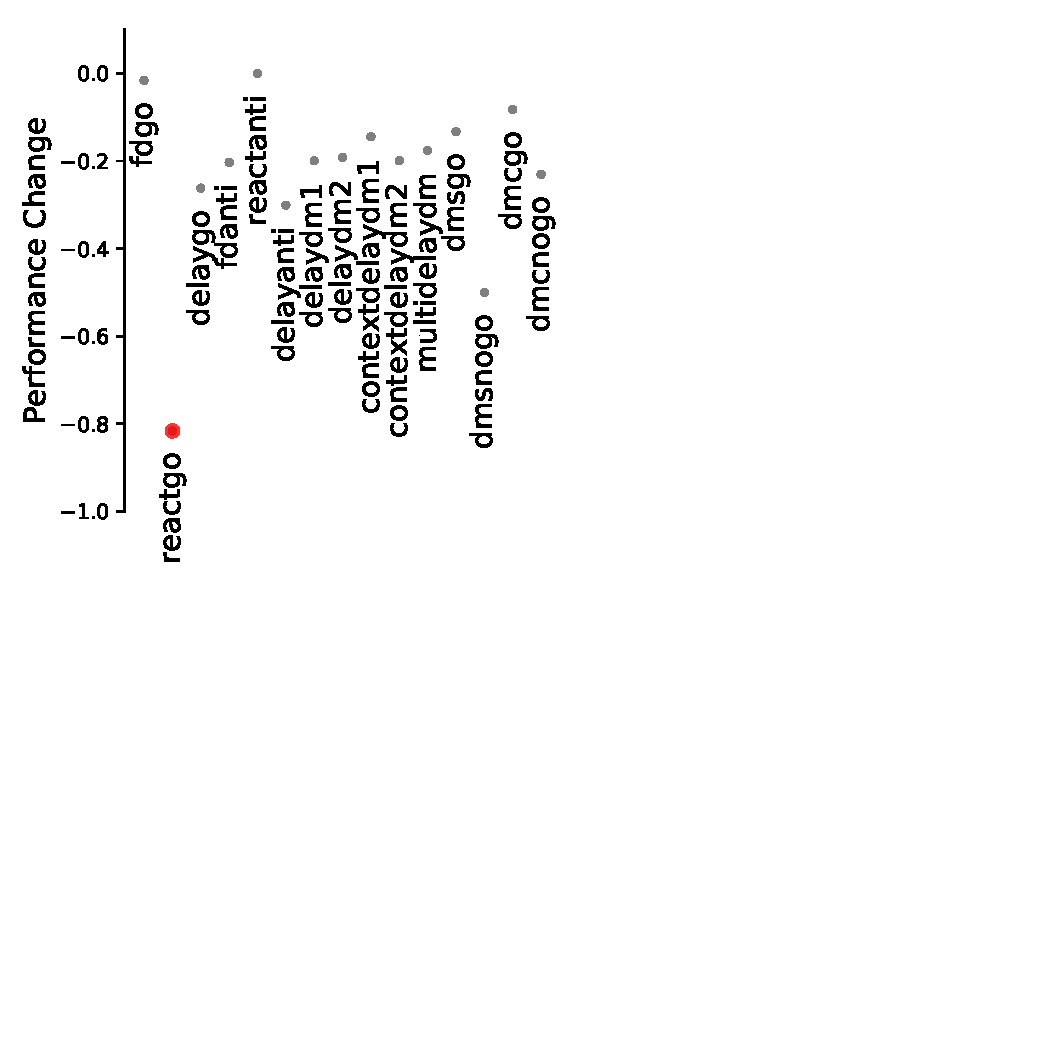
\includegraphics[trim=0mm 50mm 0mm 0mm, clip, width=0.4\linewidth]{figs/lesion \x/perf_change.pdf}};	
    \node[anchor=north] (hdiff) at ([shift={(2,2)}]perf.east) {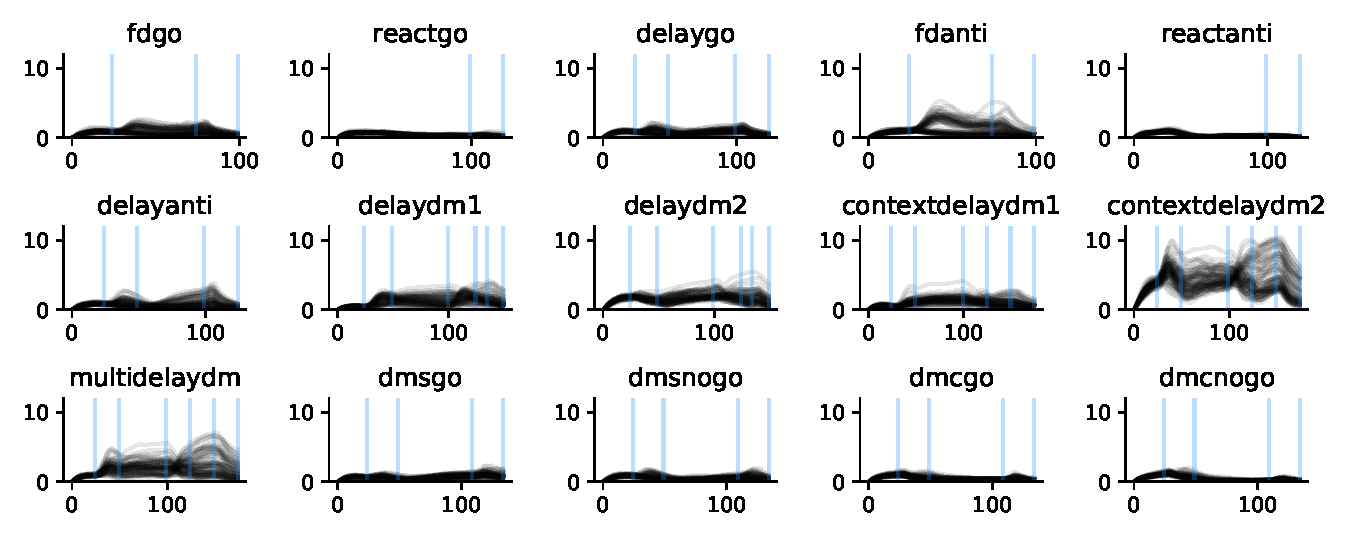
\includegraphics[trim=0mm 0mm 0mm 0mm, clip,width=0.6\linewidth]{figs/lesion \x/h_diff.pdf}};
    \node[anchor=north] (single) at ([shift={(0,0)}]perf.south) {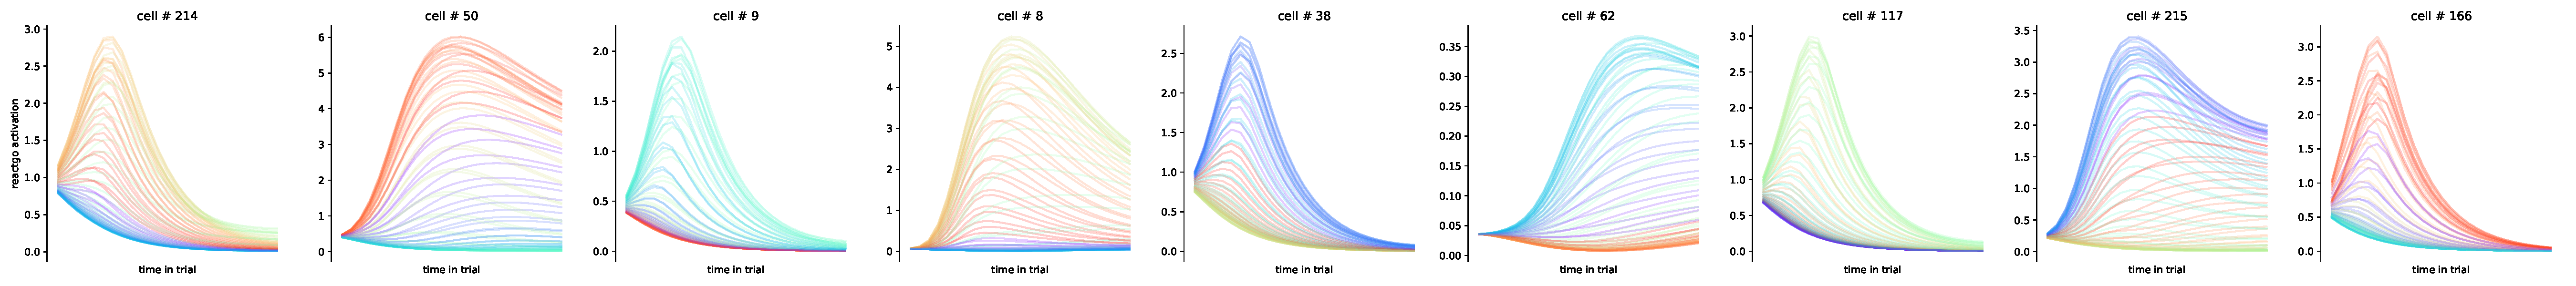
\includegraphics[trim=10mm 0mm 10mm 0mm, clip, width=0.49\linewidth]{figs/lesion \x/single_unit_activations.pdf}};
    \node[anchor=north] (pop) at ([shift={(1.5,0)}]hdiff.south) {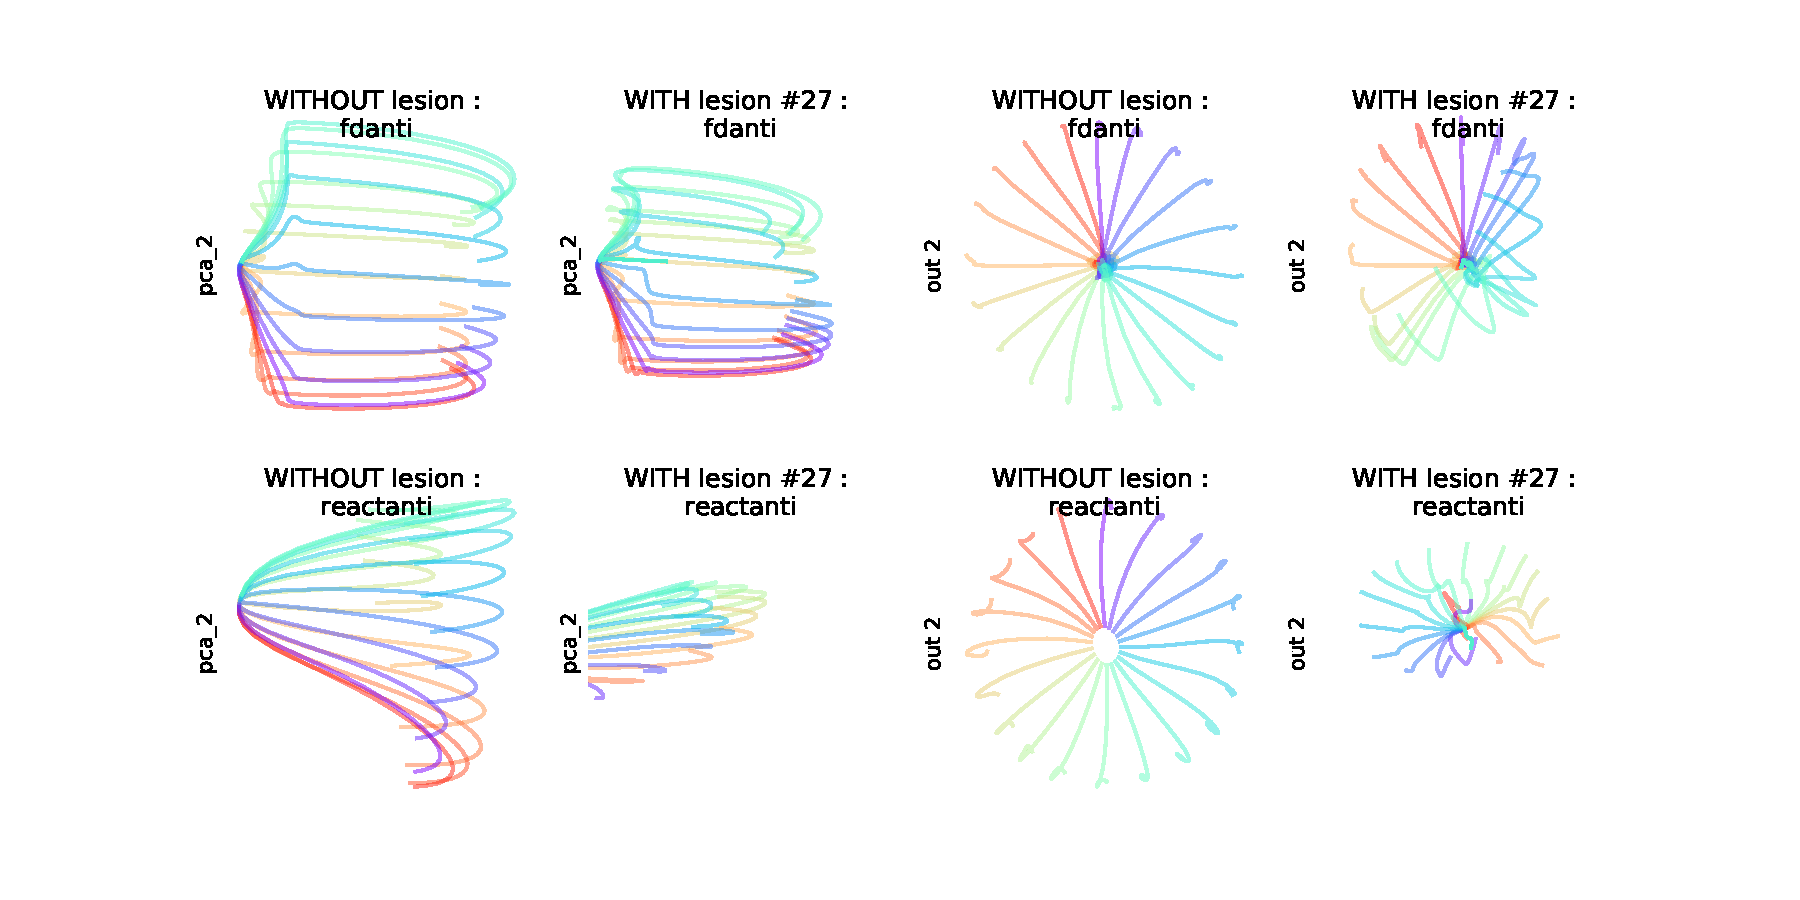
\includegraphics[trim=40mm 0mm 40mm 0mm, clip,width=0.35\linewidth]{figs/lesion \x/population_compare.pdf}};
    \node[anchor=north] (pccontribution) at ([shift={(2,0)}]single.south) {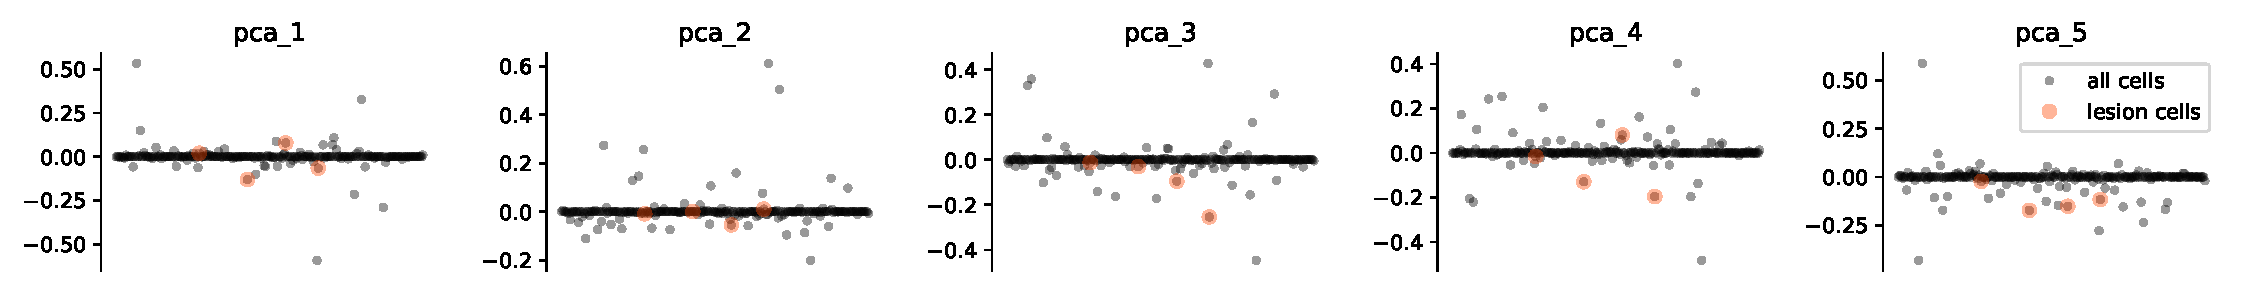
\includegraphics[trim=0mm 0mm 0mm 0mm, clip,width=0.65\linewidth]{figs/lesion \x/pc_contribution.pdf}};
    \end{tikzpicture}
    \end{figure}
    \pagebreak
}

\end{document}
